\documentclass[twoside]{book}

% Packages required by doxygen
\usepackage{fixltx2e}
\usepackage{calc}
\usepackage{doxygen}
\usepackage[export]{adjustbox} % also loads graphicx
\usepackage{graphicx}
\usepackage[utf8]{inputenc}
\usepackage{makeidx}
\usepackage{multicol}
\usepackage{multirow}
\PassOptionsToPackage{warn}{textcomp}
\usepackage{textcomp}
\usepackage[nointegrals]{wasysym}
\usepackage[table]{xcolor}

% Font selection
\usepackage[T1]{fontenc}
\usepackage[scaled=.90]{helvet}
\usepackage{courier}
\usepackage{amssymb}
\usepackage{sectsty}
\renewcommand{\familydefault}{\sfdefault}
\allsectionsfont{%
  \fontseries{bc}\selectfont%
  \color{darkgray}%
}
\renewcommand{\DoxyLabelFont}{%
  \fontseries{bc}\selectfont%
  \color{darkgray}%
}
\newcommand{\+}{\discretionary{\mbox{\scriptsize$\hookleftarrow$}}{}{}}

% Page & text layout
\usepackage{geometry}
\geometry{%
  a4paper,%
  top=2.5cm,%
  bottom=2.5cm,%
  left=2.5cm,%
  right=2.5cm%
}
\tolerance=750
\hfuzz=15pt
\hbadness=750
\setlength{\emergencystretch}{15pt}
\setlength{\parindent}{0cm}
\setlength{\parskip}{3ex plus 2ex minus 2ex}
\makeatletter
\renewcommand{\paragraph}{%
  \@startsection{paragraph}{4}{0ex}{-1.0ex}{1.0ex}{%
    \normalfont\normalsize\bfseries\SS@parafont%
  }%
}
\renewcommand{\subparagraph}{%
  \@startsection{subparagraph}{5}{0ex}{-1.0ex}{1.0ex}{%
    \normalfont\normalsize\bfseries\SS@subparafont%
  }%
}
\makeatother

% Headers & footers
\usepackage{fancyhdr}
\pagestyle{fancyplain}
\fancyhead[LE]{\fancyplain{}{\bfseries\thepage}}
\fancyhead[CE]{\fancyplain{}{}}
\fancyhead[RE]{\fancyplain{}{\bfseries\leftmark}}
\fancyhead[LO]{\fancyplain{}{\bfseries\rightmark}}
\fancyhead[CO]{\fancyplain{}{}}
\fancyhead[RO]{\fancyplain{}{\bfseries\thepage}}
\fancyfoot[LE]{\fancyplain{}{}}
\fancyfoot[CE]{\fancyplain{}{}}
\fancyfoot[RE]{\fancyplain{}{\bfseries\scriptsize Generated by Doxygen }}
\fancyfoot[LO]{\fancyplain{}{\bfseries\scriptsize Generated by Doxygen }}
\fancyfoot[CO]{\fancyplain{}{}}
\fancyfoot[RO]{\fancyplain{}{}}
\renewcommand{\footrulewidth}{0.4pt}
\renewcommand{\chaptermark}[1]{%
  \markboth{#1}{}%
}
\renewcommand{\sectionmark}[1]{%
  \markright{\thesection\ #1}%
}

% Indices & bibliography
\usepackage{natbib}
\usepackage[titles]{tocloft}
\setcounter{tocdepth}{3}
\setcounter{secnumdepth}{5}
\makeindex

% Hyperlinks (required, but should be loaded last)
\usepackage{ifpdf}
\ifpdf
  \usepackage[pdftex,pagebackref=true]{hyperref}
\else
  \usepackage[ps2pdf,pagebackref=true]{hyperref}
\fi
\hypersetup{%
  colorlinks=true,%
  linkcolor=blue,%
  citecolor=blue,%
  unicode%
}

% Custom commands
\newcommand{\clearemptydoublepage}{%
  \newpage{\pagestyle{empty}\cleardoublepage}%
}

\usepackage{caption}
\captionsetup{labelsep=space,justification=centering,font={bf},singlelinecheck=off,skip=4pt,position=top}

%===== C O N T E N T S =====

\begin{document}

% Titlepage & ToC
\hypersetup{pageanchor=false,
             bookmarksnumbered=true,
             pdfencoding=unicode
            }
\pagenumbering{alph}
\begin{titlepage}
\vspace*{7cm}
\begin{center}%
{\Large E\+D\+Bike Sensor Actuator Unit \\[1ex]\large 2 }\\
\vspace*{1cm}
{\large Generated by Doxygen 1.8.13}\\
\end{center}
\end{titlepage}
\clearemptydoublepage
\pagenumbering{roman}
\tableofcontents
\clearemptydoublepage
\pagenumbering{arabic}
\hypersetup{pageanchor=true}

%--- Begin generated contents ---
\chapter{Bug List}
\label{bug}
\Hypertarget{bug}

\begin{DoxyRefList}
\item[\label{bug__bug000001}%
\Hypertarget{bug__bug000001}%
File \hyperlink{DataBase_8cpp}{Data\+Base.cpp} ]Hvis vi sletter en tur der ikke findes forsvinder hele Data\+Basen.  
\item[\label{bug__bug000002}%
\Hypertarget{bug__bug000002}%
File \hyperlink{DataBase_8hpp}{Data\+Base.hpp} ]Hvis vi sletter en tur der ikke findes forsvinder hele Data\+Basen.  
\item[\label{bug__bug000003}%
\Hypertarget{bug__bug000003}%
File \hyperlink{EDBikeMain_8cpp}{E\+D\+Bike\+Main.cpp} ]Ingen kendte bugs.  
\item[\label{bug__bug000006}%
\Hypertarget{bug__bug000006}%
File \hyperlink{Message_8hpp}{Message.hpp} ]Ingen kendte bugs.  
\item[\label{bug__bug000007}%
\Hypertarget{bug__bug000007}%
File \hyperlink{MessageQ_8hpp}{MessageQ.hpp} ]Ingen kendte bugs.  
\item[\label{bug__bug000008}%
\Hypertarget{bug__bug000008}%
File \hyperlink{RideData_8cpp}{Ride\+Data.cpp} ]Ingen kendte bugs.  
\item[\label{bug__bug000009}%
\Hypertarget{bug__bug000009}%
File \hyperlink{RideData_8hpp}{Ride\+Data.hpp} ]Ingen kendte bugs.  
\item[\label{bug__bug000020}%
\Hypertarget{bug__bug000020}%
File \hyperlink{UserInterface_8cpp}{User\+Interface.cpp} ]Det er muligt at indstille hjulstørrelsen til 0  
\item[\label{bug__bug000021}%
\Hypertarget{bug__bug000021}%
File \hyperlink{UserInterface_8hpp}{User\+Interface.hpp} ]Det er muligt at indstille hjulstørrelsen til 0 
\end{DoxyRefList}
\chapter{File Index}
\section{File List}
Here is a list of all documented files with brief descriptions\+:\begin{DoxyCompactList}
\item\contentsline{section}{{\bfseries .\+atom-\/beautify.\+User\+Interface.\+hpp} }{\pageref{_8atom-beautify_8UserInterface_8hpp}}{}
\item\contentsline{section}{\hyperlink{DataBase_8cpp}{Data\+Base.\+cpp} \\*Implementering af Data\+Basen }{\pageref{DataBase_8cpp}}{}
\item\contentsline{section}{\hyperlink{DataBase_8hpp}{Data\+Base.\+hpp} \\*Funktionsprototyper til Data\+Basen }{\pageref{DataBase_8hpp}}{}
\item\contentsline{section}{\hyperlink{EDBikeMain_8cpp}{E\+D\+Bike\+Main.\+cpp} \\*Main-\/programmet for E\+D\+Bike }{\pageref{EDBikeMain_8cpp}}{}
\item\contentsline{section}{{\bfseries E\+D\+Bike\+Protocol.\+hpp} }{\pageref{EDBikeProtocol_8hpp}}{}
\item\contentsline{section}{{\bfseries Lock\+Unit.\+hpp} }{\pageref{LockUnit_8hpp}}{}
\item\contentsline{section}{\hyperlink{Message_8hpp}{Message.\+hpp} \\*Implementation af Message-\/klassen Denne klasse implementerer en Message-\/klasse, der bruges som base-\/class til beskederne i systemet }{\pageref{Message_8hpp}}{}
\item\contentsline{section}{\hyperlink{MessageQ_8hpp}{Message\+Q.\+hpp} \\*Implementation af Message\+Q-\/klassen Denne klasse implementerer en Message\+Queue, der bruges til at kommunikere mellem trådene i programmet }{\pageref{MessageQ_8hpp}}{}
\item\contentsline{section}{\hyperlink{RideData_8cpp}{Ride\+Data.\+cpp} \\*Implementering af \hyperlink{classRideData}{Ride\+Data} }{\pageref{RideData_8cpp}}{}
\item\contentsline{section}{\hyperlink{RideData_8hpp}{Ride\+Data.\+hpp} \\*Funktionsprototyper til \hyperlink{classRideData}{Ride\+Data} }{\pageref{RideData_8hpp}}{}
\item\contentsline{section}{{\bfseries Sensor\+Unit.\+hpp} }{\pageref{SensorUnit_8hpp}}{}
\item\contentsline{section}{{\bfseries Serial\+Unit.\+hpp} }{\pageref{SerialUnit_8hpp}}{}
\item\contentsline{section}{{\bfseries S\+P\+I.\+hpp} }{\pageref{SPI_8hpp}}{}
\item\contentsline{section}{{\bfseries S\+P\+Iprotocol.\+hpp} }{\pageref{SPIprotocol_8hpp}}{}
\item\contentsline{section}{{\bfseries thread\+Functionality.\+hpp} }{\pageref{threadFunctionality_8hpp}}{}
\item\contentsline{section}{\hyperlink{UserInterface_8cpp}{User\+Interface.\+cpp} \\*Implementation af \hyperlink{classUserInterface}{User\+Interface} }{\pageref{UserInterface_8cpp}}{}
\item\contentsline{section}{\hyperlink{UserInterface_8hpp}{User\+Interface.\+hpp} \\*Funktionsprototyper til User\+Interface-\/klassen }{\pageref{UserInterface_8hpp}}{}
\end{DoxyCompactList}

\chapter{File Documentation}
\hypertarget{Accelerometer_8h}{}\section{Accelerometer.\+h File Reference}
\label{Accelerometer_8h}\index{Accelerometer.\+h@{Accelerometer.\+h}}


Funktions implementering til accelerometeret.  


{\ttfamily \#include \char`\"{}project.\+h\char`\"{}}\newline
Include dependency graph for Accelerometer.\+h\+:
\nopagebreak
\begin{figure}[H]
\begin{center}
\leavevmode
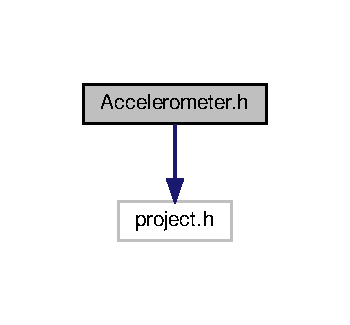
\includegraphics[width=168pt]{Accelerometer_8h__incl}
\end{center}
\end{figure}
This graph shows which files directly or indirectly include this file\+:
\nopagebreak
\begin{figure}[H]
\begin{center}
\leavevmode
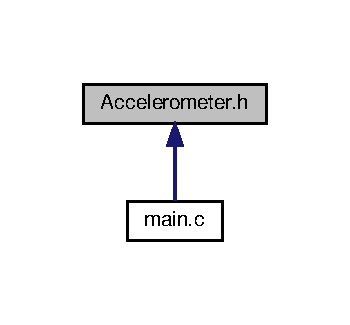
\includegraphics[width=168pt]{Accelerometer_8h__dep__incl}
\end{center}
\end{figure}
\subsection*{Functions}
\begin{DoxyCompactItemize}
\item 
\mbox{\Hypertarget{Accelerometer_8h_aedd212ed9cb67e88387fee6a77e97187}\label{Accelerometer_8h_aedd212ed9cb67e88387fee6a77e97187}} 
void \hyperlink{Accelerometer_8h_aedd212ed9cb67e88387fee6a77e97187}{init\+\_\+accelerometer} ()
\begin{DoxyCompactList}\small\item\em Init funktion til accelerometeret. Initiere interrupt rutinerne, som er forbundet med accelerometeret. \end{DoxyCompactList}\item 
void \hyperlink{Accelerometer_8h_a5c823e0fb40fe73ee218325d6830e16f}{stop\+Accelerometer\+Timer} ()
\begin{DoxyCompactList}\small\item\em Stopper accelerometerets timer. \end{DoxyCompactList}\item 
void \hyperlink{Accelerometer_8h_ac015f7f6e3a104f94f1b6a862709aaf0}{start\+Accelerometer\+Timer} ()
\begin{DoxyCompactList}\small\item\em Starter accelerometerets timer. \end{DoxyCompactList}\item 
void \hyperlink{Accelerometer_8h_a67004092d5193d69d00f8b936e49ad16}{reset\+Accelerometer\+Timer} ()
\begin{DoxyCompactList}\small\item\em resetter accelerometerets timer \end{DoxyCompactList}\end{DoxyCompactItemize}


\subsection{Detailed Description}
Funktions implementering til accelerometeret. 

Funktions og interrupt prototyper til accelerometeret.

Indeholder implementeringer af funktionerne fra accelerometer.\+h

\begin{DoxyAuthor}{Author}
Jonathan Hartvigsen Juncker 

Frederik Runge-\/\+Dalager 
\end{DoxyAuthor}
\begin{DoxyRefDesc}{Bug}
\item[\hyperlink{bug__bug000001}{Bug}]Ingen kendte bugs. \end{DoxyRefDesc}


Indeholder prototyperne til interrupt handlers som relaterer til accelerometeret og funktions prototyperne til Accelerometer.\+c

\begin{DoxyAuthor}{Author}
Jonathan Hartvigsen Juncker 

Frederik Runge-\/\+Dalager 
\end{DoxyAuthor}
\begin{DoxyRefDesc}{Bug}
\item[\hyperlink{bug__bug000002}{Bug}]Ingen kendte bugs. \end{DoxyRefDesc}


\subsection{Function Documentation}
\mbox{\Hypertarget{Accelerometer_8h_a67004092d5193d69d00f8b936e49ad16}\label{Accelerometer_8h_a67004092d5193d69d00f8b936e49ad16}} 
\index{Accelerometer.\+h@{Accelerometer.\+h}!reset\+Accelerometer\+Timer@{reset\+Accelerometer\+Timer}}
\index{reset\+Accelerometer\+Timer@{reset\+Accelerometer\+Timer}!Accelerometer.\+h@{Accelerometer.\+h}}
\subsubsection{\texorpdfstring{reset\+Accelerometer\+Timer()}{resetAccelerometerTimer()}}
{\footnotesize\ttfamily void reset\+Accelerometer\+Timer (\begin{DoxyParamCaption}{ }\end{DoxyParamCaption})}



resetter accelerometerets timer 

\mbox{\Hypertarget{Accelerometer_8h_ac015f7f6e3a104f94f1b6a862709aaf0}\label{Accelerometer_8h_ac015f7f6e3a104f94f1b6a862709aaf0}} 
\index{Accelerometer.\+h@{Accelerometer.\+h}!start\+Accelerometer\+Timer@{start\+Accelerometer\+Timer}}
\index{start\+Accelerometer\+Timer@{start\+Accelerometer\+Timer}!Accelerometer.\+h@{Accelerometer.\+h}}
\subsubsection{\texorpdfstring{start\+Accelerometer\+Timer()}{startAccelerometerTimer()}}
{\footnotesize\ttfamily void start\+Accelerometer\+Timer (\begin{DoxyParamCaption}{ }\end{DoxyParamCaption})}



Starter accelerometerets timer. 

\mbox{\Hypertarget{Accelerometer_8h_a5c823e0fb40fe73ee218325d6830e16f}\label{Accelerometer_8h_a5c823e0fb40fe73ee218325d6830e16f}} 
\index{Accelerometer.\+h@{Accelerometer.\+h}!stop\+Accelerometer\+Timer@{stop\+Accelerometer\+Timer}}
\index{stop\+Accelerometer\+Timer@{stop\+Accelerometer\+Timer}!Accelerometer.\+h@{Accelerometer.\+h}}
\subsubsection{\texorpdfstring{stop\+Accelerometer\+Timer()}{stopAccelerometerTimer()}}
{\footnotesize\ttfamily void stop\+Accelerometer\+Timer (\begin{DoxyParamCaption}{ }\end{DoxyParamCaption})}



Stopper accelerometerets timer. 


\hypertarget{lockUnit_8c}{}\section{lock\+Unit.\+c File Reference}
\label{lockUnit_8c}\index{lock\+Unit.\+c@{lock\+Unit.\+c}}


funktions implementeringer til låsen  


{\ttfamily \#include \char`\"{}lock\+Unit.\+h\char`\"{}}\newline
{\ttfamily \#include \char`\"{}E\+D\+Bike\+Protocol.\+h\char`\"{}}\newline
Include dependency graph for lock\+Unit.\+c\+:
\nopagebreak
\begin{figure}[H]
\begin{center}
\leavevmode
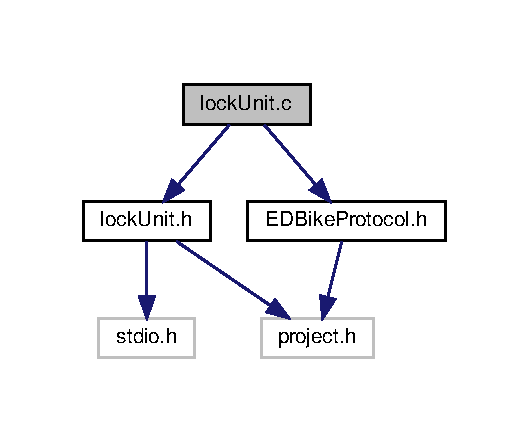
\includegraphics[width=254pt]{lockUnit_8c__incl}
\end{center}
\end{figure}
\subsection*{Functions}
\begin{DoxyCompactItemize}
\item 
\mbox{\Hypertarget{lockUnit_8c_ae42548961b3afb4d6eda673e595f37d8}\label{lockUnit_8c_ae42548961b3afb4d6eda673e595f37d8}} 
void \hyperlink{lockUnit_8c_ae42548961b3afb4d6eda673e595f37d8}{init\+Lock\+Unit} ()
\begin{DoxyCompactList}\small\item\em Init funktion til låsen. Initiere interrupt rutinerne, som er forbundet med låsen. \end{DoxyCompactList}\item 
\mbox{\Hypertarget{lockUnit_8c_a732e06dbf599e5ea946a66afe3ca0ed2}\label{lockUnit_8c_a732e06dbf599e5ea946a66afe3ca0ed2}} 
void \hyperlink{lockUnit_8c_a732e06dbf599e5ea946a66afe3ca0ed2}{unlock\+Bike} ()
\begin{DoxyCompactList}\small\item\em Unlock funktion til låsen. Låser låsen op og tænder for motor timeren. \end{DoxyCompactList}\item 
\mbox{\Hypertarget{lockUnit_8c_ac801da6dcc1e4d828951c4f20d3b7631}\label{lockUnit_8c_ac801da6dcc1e4d828951c4f20d3b7631}} 
void \hyperlink{lockUnit_8c_ac801da6dcc1e4d828951c4f20d3b7631}{lock\+Bike} ()
\begin{DoxyCompactList}\small\item\em lock funktion til låsen. Låser låsen og tænder for motor timeren. \end{DoxyCompactList}\item 
\mbox{\Hypertarget{lockUnit_8c_a5ee55fea0a10de0b232db271f0ee2c15}\label{lockUnit_8c_a5ee55fea0a10de0b232db271f0ee2c15}} 
void \hyperlink{lockUnit_8c_a5ee55fea0a10de0b232db271f0ee2c15}{stop\+Lock\+Timer} ()
\begin{DoxyCompactList}\small\item\em Stop funktion til motor timeren. Stopper motor timeren. \end{DoxyCompactList}\end{DoxyCompactItemize}


\subsection{Detailed Description}
funktions implementeringer til låsen 

Indeholder implementeringer af funktionerne fra \hyperlink{lockUnit_8h}{lock\+Unit.\+h}

\begin{DoxyAuthor}{Author}
Jonathan Hartvigsen Juncker 

Mortada Ismail 
\end{DoxyAuthor}
\begin{DoxyRefDesc}{Bug}
\item[\hyperlink{bug__bug000003}{Bug}]Ingen kendte bugs. \end{DoxyRefDesc}

\hypertarget{lockUnit_8h}{}\section{lock\+Unit.\+h File Reference}
\label{lockUnit_8h}\index{lock\+Unit.\+h@{lock\+Unit.\+h}}


Funktions og interrupt prototyper til låsen.  


{\ttfamily \#include $<$stdio.\+h$>$}\newline
{\ttfamily \#include \char`\"{}project.\+h\char`\"{}}\newline
Include dependency graph for lock\+Unit.\+h\+:
\nopagebreak
\begin{figure}[H]
\begin{center}
\leavevmode
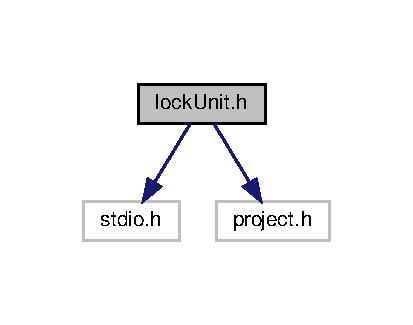
\includegraphics[width=198pt]{lockUnit_8h__incl}
\end{center}
\end{figure}
This graph shows which files directly or indirectly include this file\+:
\nopagebreak
\begin{figure}[H]
\begin{center}
\leavevmode
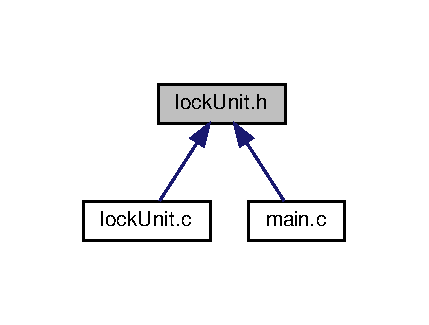
\includegraphics[width=206pt]{lockUnit_8h__dep__incl}
\end{center}
\end{figure}
\subsection*{Functions}
\begin{DoxyCompactItemize}
\item 
\mbox{\Hypertarget{lockUnit_8h_ae42548961b3afb4d6eda673e595f37d8}\label{lockUnit_8h_ae42548961b3afb4d6eda673e595f37d8}} 
void \hyperlink{lockUnit_8h_ae42548961b3afb4d6eda673e595f37d8}{init\+Lock\+Unit} ()
\begin{DoxyCompactList}\small\item\em Init funktion til låsen. Initiere interrupt rutinerne, som er forbundet med låsen. \end{DoxyCompactList}\item 
\mbox{\Hypertarget{lockUnit_8h_a732e06dbf599e5ea946a66afe3ca0ed2}\label{lockUnit_8h_a732e06dbf599e5ea946a66afe3ca0ed2}} 
void \hyperlink{lockUnit_8h_a732e06dbf599e5ea946a66afe3ca0ed2}{unlock\+Bike} ()
\begin{DoxyCompactList}\small\item\em Unlock funktion til låsen. Låser låsen op og tænder for motor timeren. \end{DoxyCompactList}\item 
\mbox{\Hypertarget{lockUnit_8h_ac801da6dcc1e4d828951c4f20d3b7631}\label{lockUnit_8h_ac801da6dcc1e4d828951c4f20d3b7631}} 
void \hyperlink{lockUnit_8h_ac801da6dcc1e4d828951c4f20d3b7631}{lock\+Bike} ()
\begin{DoxyCompactList}\small\item\em lock funktion til låsen. Låser låsen og tænder for motor timeren. \end{DoxyCompactList}\item 
\mbox{\Hypertarget{lockUnit_8h_a5ee55fea0a10de0b232db271f0ee2c15}\label{lockUnit_8h_a5ee55fea0a10de0b232db271f0ee2c15}} 
void \hyperlink{lockUnit_8h_a5ee55fea0a10de0b232db271f0ee2c15}{stop\+Lock\+Timer} ()
\begin{DoxyCompactList}\small\item\em Stop funktion til motor timeren. Stopper motor timeren. \end{DoxyCompactList}\end{DoxyCompactItemize}


\subsection{Detailed Description}
Funktions og interrupt prototyper til låsen. 

Indeholder prototyperne til interrupt handlers som relaterer til låsen og funktions prototyperne til \hyperlink{lockUnit_8c}{lock\+Unit.\+c}

\begin{DoxyAuthor}{Author}
Jonathan Hartvigsen Juncker 

Mortada Ismail 
\end{DoxyAuthor}
\begin{DoxyRefDesc}{Bug}
\item[\hyperlink{bug__bug000004}{Bug}]Ingen kendte bugs. \end{DoxyRefDesc}

\hypertarget{main_8c}{}\section{main.\+c File Reference}
\label{main_8c}\index{main.\+c@{main.\+c}}


P\+SoC main.  


{\ttfamily \#include $<$stdio.\+h$>$}\newline
{\ttfamily \#include \char`\"{}project.\+h\char`\"{}}\newline
{\ttfamily \#include \char`\"{}E\+D\+Bike\+Protocol.\+h\char`\"{}}\newline
{\ttfamily \#include \char`\"{}lock\+Unit.\+h\char`\"{}}\newline
{\ttfamily \#include \char`\"{}S\+P\+I.\+h\char`\"{}}\newline
{\ttfamily \#include \char`\"{}wheel\+Sensor.\+h\char`\"{}}\newline
{\ttfamily \#include \char`\"{}Accelerometer.\+h\char`\"{}}\newline
{\ttfamily \#include \char`\"{}U\+A\+R\+T.\+h\char`\"{}}\newline
{\ttfamily \#include \char`\"{}bike\+State.\+h\char`\"{}}\newline
{\ttfamily \#include \char`\"{}S\+P\+Iprotocol.\+h\char`\"{}}\newline
Include dependency graph for main.\+c\+:
\nopagebreak
\begin{figure}[H]
\begin{center}
\leavevmode
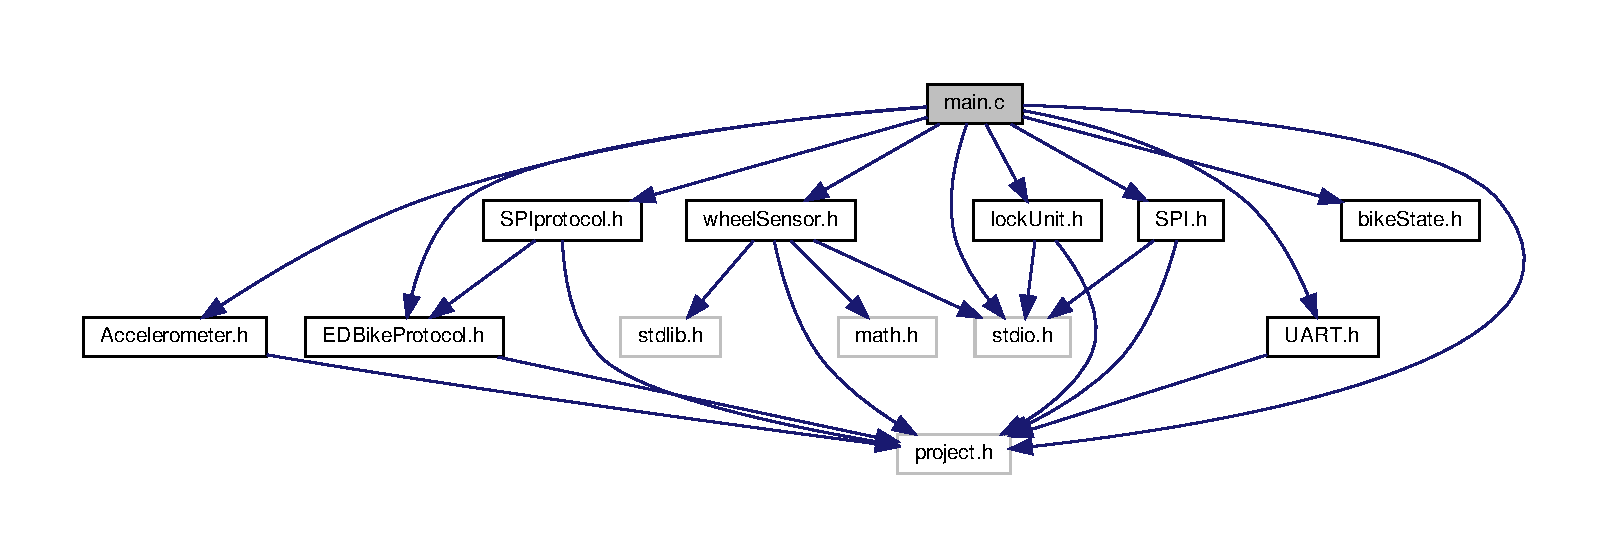
\includegraphics[width=350pt]{main_8c__incl}
\end{center}
\end{figure}


\subsection{Detailed Description}
P\+SoC main. 

\begin{DoxyAuthor}{Author}
Jonathan Hartvigsen Juncker 

Kristian Lau Jespersen 
\end{DoxyAuthor}
\begin{DoxyRefDesc}{Bug}
\item[\hyperlink{bug__bug000005}{Bug}]Ingen kendte bugs. \end{DoxyRefDesc}

\hypertarget{SPI_8c}{}\section{S\+P\+I.\+c File Reference}
\label{SPI_8c}\index{S\+P\+I.\+c@{S\+P\+I.\+c}}


funktions implementeringer til S\+PI kommunikation  


{\ttfamily \#include \char`\"{}S\+P\+I.\+h\char`\"{}}\newline
Include dependency graph for S\+P\+I.\+c\+:
\nopagebreak
\begin{figure}[H]
\begin{center}
\leavevmode
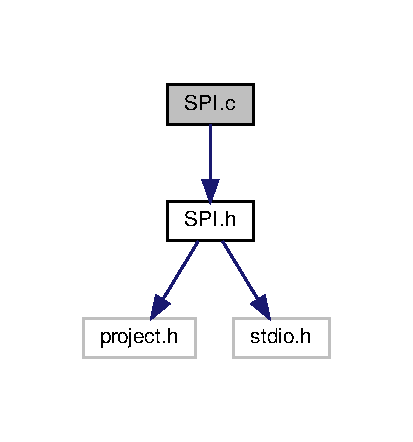
\includegraphics[width=198pt]{SPI_8c__incl}
\end{center}
\end{figure}
\subsection*{Functions}
\begin{DoxyCompactItemize}
\item 
\mbox{\Hypertarget{SPI_8c_a070402cc6c1cae693d10f59f9c483f76}\label{SPI_8c_a070402cc6c1cae693d10f59f9c483f76}} 
void \hyperlink{SPI_8c_a070402cc6c1cae693d10f59f9c483f76}{init\+S\+PI} ()
\begin{DoxyCompactList}\small\item\em Init funktion til låsen. Initiere interrupt rutinerne som er forbundet med S\+PI, og tømmer F\+I\+FO\textquotesingle{}en og starter S\+PI komponenten. \end{DoxyCompactList}\item 
\mbox{\Hypertarget{SPI_8c_aa7447a8d9d037be043d4ac67d91b099c}\label{SPI_8c_aa7447a8d9d037be043d4ac67d91b099c}} 
void \hyperlink{SPI_8c_aa7447a8d9d037be043d4ac67d91b099c}{terminate\+S\+PI} ()
\begin{DoxyCompactList}\small\item\em Stop funktion til S\+PI komponenten. Slukker S\+PI Komponenten. \end{DoxyCompactList}\item 
void \hyperlink{SPI_8c_abac47ea38c38eb86456d9d41752778bb}{receive\+S\+PI} (uint8 $\ast$rx\+Buffer)
\begin{DoxyCompactList}\small\item\em Funktion til modtagelse af information fra S\+P\+I-\/\+Master. Læser fra rx bufferen. \end{DoxyCompactList}\item 
void \hyperlink{SPI_8c_a5d180e90614c451cdd2cfe65c6875963}{load\+To\+Specific\+Tx\+Buffer\+Index} (uint8 $\ast$tx\+Buffer, uint8 index, uint8 data)
\begin{DoxyCompactList}\small\item\em Funktion til indlæsning af information til tx S\+P\+I-\/masteren Indlæser information til tx bufferen. \end{DoxyCompactList}\item 
void \hyperlink{SPI_8c_af3ae4b62f31497bf152aa1008a266d75}{transfer\+Is\+Ready} (uint8 $\ast$tx\+Buffer)
\begin{DoxyCompactList}\small\item\em Funktion der sørger for at lægge data klar i S\+P\+I-\/enhedens F\+I\+F\+O-\/kø Når \hyperlink{SPI_8h_af3ae4b62f31497bf152aa1008a266d75}{transfer\+Is\+Ready()} kaldes med variablen tx\+Buffer som parameter, laves 5 kopier af indholdet i tx\+Buffer, hvilke placeres i den 6 gange så lange buffer tx\+Clone\+Buffer. \end{DoxyCompactList}\end{DoxyCompactItemize}


\subsection{Detailed Description}
funktions implementeringer til S\+PI kommunikation 

Indeholder implementeringer af funktionerne fra \hyperlink{SPI_8h}{S\+P\+I.\+h}

\begin{DoxyAuthor}{Author}
Kristian Lau Jespersen 
\end{DoxyAuthor}
\begin{DoxyRefDesc}{Bug}
\item[\hyperlink{bug__bug000006}{Bug}]Ingen kendte bugs. \end{DoxyRefDesc}


\subsection{Function Documentation}
\mbox{\Hypertarget{SPI_8c_a5d180e90614c451cdd2cfe65c6875963}\label{SPI_8c_a5d180e90614c451cdd2cfe65c6875963}} 
\index{S\+P\+I.\+c@{S\+P\+I.\+c}!load\+To\+Specific\+Tx\+Buffer\+Index@{load\+To\+Specific\+Tx\+Buffer\+Index}}
\index{load\+To\+Specific\+Tx\+Buffer\+Index@{load\+To\+Specific\+Tx\+Buffer\+Index}!S\+P\+I.\+c@{S\+P\+I.\+c}}
\subsubsection{\texorpdfstring{load\+To\+Specific\+Tx\+Buffer\+Index()}{loadToSpecificTxBufferIndex()}}
{\footnotesize\ttfamily void load\+To\+Specific\+Tx\+Buffer\+Index (\begin{DoxyParamCaption}\item[{uint8 $\ast$}]{tx\+Buffer,  }\item[{uint8}]{index,  }\item[{uint8}]{data }\end{DoxyParamCaption})}



Funktion til indlæsning af information til tx S\+P\+I-\/masteren Indlæser information til tx bufferen. 

tx\+Buffer bufferen hvor informationen som S\+PI slaven skal sende til S\+PI Masteren bliver lagt.


\begin{DoxyParams}{Parameters}
{\em index} & de index informationen skal indsættes i.\\
\hline
{\em data} & \\
\hline
\end{DoxyParams}
\mbox{\Hypertarget{SPI_8c_abac47ea38c38eb86456d9d41752778bb}\label{SPI_8c_abac47ea38c38eb86456d9d41752778bb}} 
\index{S\+P\+I.\+c@{S\+P\+I.\+c}!receive\+S\+PI@{receive\+S\+PI}}
\index{receive\+S\+PI@{receive\+S\+PI}!S\+P\+I.\+c@{S\+P\+I.\+c}}
\subsubsection{\texorpdfstring{receive\+S\+P\+I()}{receiveSPI()}}
{\footnotesize\ttfamily void receive\+S\+PI (\begin{DoxyParamCaption}\item[{uint8 $\ast$}]{rx\+Buffer }\end{DoxyParamCaption})}



Funktion til modtagelse af information fra S\+P\+I-\/\+Master. Læser fra rx bufferen. 


\begin{DoxyParams}{Parameters}
{\em rx\+Buffer} & bufferen hvori informationen som S\+PI masteren har sendt ligger. \\
\hline
\end{DoxyParams}
\mbox{\Hypertarget{SPI_8c_af3ae4b62f31497bf152aa1008a266d75}\label{SPI_8c_af3ae4b62f31497bf152aa1008a266d75}} 
\index{S\+P\+I.\+c@{S\+P\+I.\+c}!transfer\+Is\+Ready@{transfer\+Is\+Ready}}
\index{transfer\+Is\+Ready@{transfer\+Is\+Ready}!S\+P\+I.\+c@{S\+P\+I.\+c}}
\subsubsection{\texorpdfstring{transfer\+Is\+Ready()}{transferIsReady()}}
{\footnotesize\ttfamily void transfer\+Is\+Ready (\begin{DoxyParamCaption}\item[{uint8 $\ast$}]{tx\+Buffer }\end{DoxyParamCaption})}



Funktion der sørger for at lægge data klar i S\+P\+I-\/enhedens F\+I\+F\+O-\/kø Når \hyperlink{SPI_8h_af3ae4b62f31497bf152aa1008a266d75}{transfer\+Is\+Ready()} kaldes med variablen tx\+Buffer som parameter, laves 5 kopier af indholdet i tx\+Buffer, hvilke placeres i den 6 gange så lange buffer tx\+Clone\+Buffer. 


\begin{DoxyParams}{Parameters}
{\em tx\+Buffer} & bufferen hvor informationen som S\+PI slaven skal sende til S\+PI Masteren bliver lagt. \\
\hline
\end{DoxyParams}

\hypertarget{SPI_8h}{}\section{S\+P\+I.\+h File Reference}
\label{SPI_8h}\index{S\+P\+I.\+h@{S\+P\+I.\+h}}


Funktions og interrupt prototyper til S\+PI kommunikation.  


{\ttfamily \#include \char`\"{}project.\+h\char`\"{}}\newline
{\ttfamily \#include $<$stdio.\+h$>$}\newline
Include dependency graph for S\+P\+I.\+h\+:
\nopagebreak
\begin{figure}[H]
\begin{center}
\leavevmode
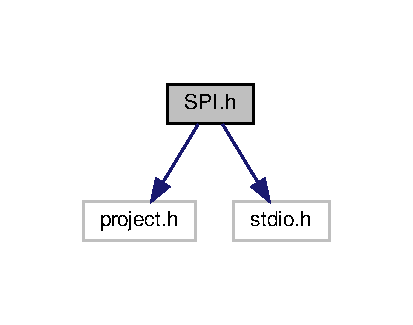
\includegraphics[width=198pt]{SPI_8h__incl}
\end{center}
\end{figure}
This graph shows which files directly or indirectly include this file\+:
\nopagebreak
\begin{figure}[H]
\begin{center}
\leavevmode
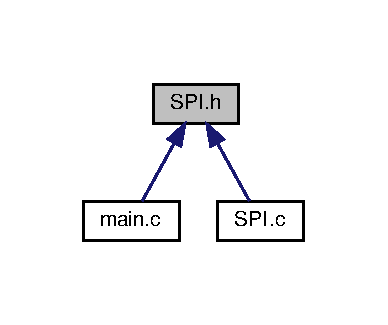
\includegraphics[width=186pt]{SPI_8h__dep__incl}
\end{center}
\end{figure}
\subsection*{Functions}
\begin{DoxyCompactItemize}
\item 
\mbox{\Hypertarget{SPI_8h_a070402cc6c1cae693d10f59f9c483f76}\label{SPI_8h_a070402cc6c1cae693d10f59f9c483f76}} 
void \hyperlink{SPI_8h_a070402cc6c1cae693d10f59f9c483f76}{init\+S\+PI} ()
\begin{DoxyCompactList}\small\item\em Init funktion til låsen. Initiere interrupt rutinerne som er forbundet med S\+PI, og tømmer F\+I\+FO\textquotesingle{}en og starter S\+PI komponenten. \end{DoxyCompactList}\item 
\mbox{\Hypertarget{SPI_8h_aa7447a8d9d037be043d4ac67d91b099c}\label{SPI_8h_aa7447a8d9d037be043d4ac67d91b099c}} 
void \hyperlink{SPI_8h_aa7447a8d9d037be043d4ac67d91b099c}{terminate\+S\+PI} ()
\begin{DoxyCompactList}\small\item\em Stop funktion til S\+PI komponenten. Slukker S\+PI Komponenten. \end{DoxyCompactList}\item 
void \hyperlink{SPI_8h_abac47ea38c38eb86456d9d41752778bb}{receive\+S\+PI} (uint8 $\ast$rx\+Buffer)
\begin{DoxyCompactList}\small\item\em Funktion til modtagelse af information fra S\+P\+I-\/\+Master. Læser fra rx bufferen. \end{DoxyCompactList}\item 
void \hyperlink{SPI_8h_a5d180e90614c451cdd2cfe65c6875963}{load\+To\+Specific\+Tx\+Buffer\+Index} (uint8 $\ast$tx\+Buffer, uint8 index, uint8 data)
\begin{DoxyCompactList}\small\item\em Funktion til indlæsning af information til tx S\+P\+I-\/masteren Indlæser information til tx bufferen. \end{DoxyCompactList}\item 
void \hyperlink{SPI_8h_af3ae4b62f31497bf152aa1008a266d75}{transfer\+Is\+Ready} (uint8 $\ast$tx\+Buffer)
\begin{DoxyCompactList}\small\item\em Funktion der sørger for at lægge data klar i S\+P\+I-\/enhedens F\+I\+F\+O-\/kø Når \hyperlink{SPI_8h_af3ae4b62f31497bf152aa1008a266d75}{transfer\+Is\+Ready()} kaldes med variablen tx\+Buffer som parameter, laves 5 kopier af indholdet i tx\+Buffer, hvilke placeres i den 6 gange så lange buffer tx\+Clone\+Buffer. \end{DoxyCompactList}\end{DoxyCompactItemize}


\subsection{Detailed Description}
Funktions og interrupt prototyper til S\+PI kommunikation. 

Indeholder prototyperne til interrupt handlers som relaterer til S\+PI og funktions prototyperne til \hyperlink{SPI_8c}{S\+P\+I.\+c}

\begin{DoxyAuthor}{Author}
Kristian Lau Jespersen 
\end{DoxyAuthor}
\begin{DoxyRefDesc}{Bug}
\item[\hyperlink{bug__bug000007}{Bug}]Ingen kendte bugs. \end{DoxyRefDesc}


Indeholder funktions prototyperne til \hyperlink{SPI_8c}{S\+P\+I.\+c}

\begin{DoxyAuthor}{Author}
Kristian Lau Jespersen 

Jonathan Hartvigsen Juncker 
\end{DoxyAuthor}
\begin{DoxyRefDesc}{Bug}
\item[\hyperlink{bug__bug000011}{Bug}]Ingen kendte bugs. \end{DoxyRefDesc}


\subsection{Function Documentation}
\mbox{\Hypertarget{SPI_8h_a5d180e90614c451cdd2cfe65c6875963}\label{SPI_8h_a5d180e90614c451cdd2cfe65c6875963}} 
\index{S\+P\+I.\+h@{S\+P\+I.\+h}!load\+To\+Specific\+Tx\+Buffer\+Index@{load\+To\+Specific\+Tx\+Buffer\+Index}}
\index{load\+To\+Specific\+Tx\+Buffer\+Index@{load\+To\+Specific\+Tx\+Buffer\+Index}!S\+P\+I.\+h@{S\+P\+I.\+h}}
\subsubsection{\texorpdfstring{load\+To\+Specific\+Tx\+Buffer\+Index()}{loadToSpecificTxBufferIndex()}}
{\footnotesize\ttfamily void load\+To\+Specific\+Tx\+Buffer\+Index (\begin{DoxyParamCaption}\item[{uint8 $\ast$}]{tx\+Buffer,  }\item[{uint8}]{index,  }\item[{uint8}]{data }\end{DoxyParamCaption})}



Funktion til indlæsning af information til tx S\+P\+I-\/masteren Indlæser information til tx bufferen. 

tx\+Buffer bufferen hvor informationen som S\+PI slaven skal sende til S\+PI Masteren bliver lagt.


\begin{DoxyParams}{Parameters}
{\em index} & de index informationen skal indsættes i.\\
\hline
{\em data} & \\
\hline
\end{DoxyParams}
\mbox{\Hypertarget{SPI_8h_abac47ea38c38eb86456d9d41752778bb}\label{SPI_8h_abac47ea38c38eb86456d9d41752778bb}} 
\index{S\+P\+I.\+h@{S\+P\+I.\+h}!receive\+S\+PI@{receive\+S\+PI}}
\index{receive\+S\+PI@{receive\+S\+PI}!S\+P\+I.\+h@{S\+P\+I.\+h}}
\subsubsection{\texorpdfstring{receive\+S\+P\+I()}{receiveSPI()}}
{\footnotesize\ttfamily void receive\+S\+PI (\begin{DoxyParamCaption}\item[{uint8 $\ast$}]{rx\+Buffer }\end{DoxyParamCaption})}



Funktion til modtagelse af information fra S\+P\+I-\/\+Master. Læser fra rx bufferen. 


\begin{DoxyParams}{Parameters}
{\em rx\+Buffer} & bufferen hvori informationen som S\+PI masteren har sendt ligger. \\
\hline
\end{DoxyParams}
\mbox{\Hypertarget{SPI_8h_af3ae4b62f31497bf152aa1008a266d75}\label{SPI_8h_af3ae4b62f31497bf152aa1008a266d75}} 
\index{S\+P\+I.\+h@{S\+P\+I.\+h}!transfer\+Is\+Ready@{transfer\+Is\+Ready}}
\index{transfer\+Is\+Ready@{transfer\+Is\+Ready}!S\+P\+I.\+h@{S\+P\+I.\+h}}
\subsubsection{\texorpdfstring{transfer\+Is\+Ready()}{transferIsReady()}}
{\footnotesize\ttfamily void transfer\+Is\+Ready (\begin{DoxyParamCaption}\item[{uint8 $\ast$}]{tx\+Buffer }\end{DoxyParamCaption})}



Funktion der sørger for at lægge data klar i S\+P\+I-\/enhedens F\+I\+F\+O-\/kø Når \hyperlink{SPI_8h_af3ae4b62f31497bf152aa1008a266d75}{transfer\+Is\+Ready()} kaldes med variablen tx\+Buffer som parameter, laves 5 kopier af indholdet i tx\+Buffer, hvilke placeres i den 6 gange så lange buffer tx\+Clone\+Buffer. 


\begin{DoxyParams}{Parameters}
{\em tx\+Buffer} & bufferen hvor informationen som S\+PI slaven skal sende til S\+PI Masteren bliver lagt. \\
\hline
\end{DoxyParams}

\hypertarget{SPIprotocol_8c}{}\section{S\+P\+Iprotocol.\+c File Reference}
\label{SPIprotocol_8c}\index{S\+P\+Iprotocol.\+c@{S\+P\+Iprotocol.\+c}}


funktions implementeringer til S\+PI kommunikation  


{\ttfamily \#include \char`\"{}S\+P\+Iprotocol.\+h\char`\"{}}\newline
Include dependency graph for S\+P\+Iprotocol.\+c\+:
\nopagebreak
\begin{figure}[H]
\begin{center}
\leavevmode
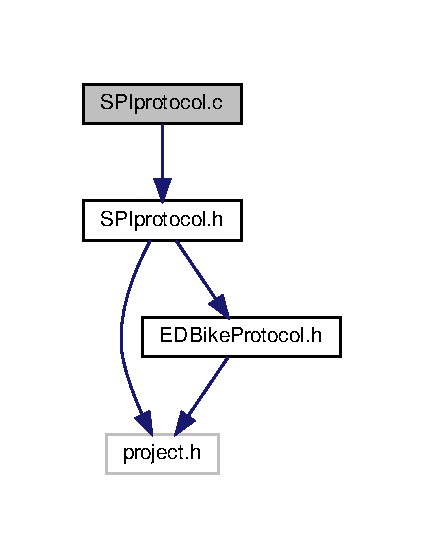
\includegraphics[width=204pt]{SPIprotocol_8c__incl}
\end{center}
\end{figure}
\subsection*{Functions}
\begin{DoxyCompactItemize}
\item 
void \hyperlink{SPIprotocol_8c_a43827de2fc968bbd1b3081e66c606cf8}{extract\+From\+Buffer} (uint8\+\_\+t $\ast$speed, uint8\+\_\+t $\ast$distance, uint8\+\_\+t $\ast$buffer)
\begin{DoxyCompactList}\small\item\em Funktion til at uddrage information fra en buffer Henter speed og distance fra rx bufferen. \end{DoxyCompactList}\item 
uint8\+\_\+t \hyperlink{SPIprotocol_8c_affe5db7b5f6fb00785f2e52d8b5462f0}{error\+Check\+With\+Odd\+Parity} (uint8\+\_\+t $\ast$buffer, uint8\+\_\+t length\+Of\+Buffer)
\begin{DoxyCompactList}\small\item\em Funktion til check af paritets bit. Checker tx/rx buffere for paritets bit. \end{DoxyCompactList}\item 
void \hyperlink{SPIprotocol_8c_a9f7556559e84f123b72eefce42c02710}{create\+Parity\+Bits} (uint8\+\_\+t $\ast$buffer, uint8\+\_\+t length\+Of\+Buffer)
\begin{DoxyCompactList}\small\item\em Funktion til kreering af paritets bits Laver paritet bits til en tx/rx buffer. \end{DoxyCompactList}\end{DoxyCompactItemize}


\subsection{Detailed Description}
funktions implementeringer til S\+PI kommunikation 

Indeholder implementeringer af funktionerne fra \hyperlink{SPIprotocol_8h}{S\+P\+Iprotocol.\+h}

\begin{DoxyAuthor}{Author}
Kristian Lau Jespersen 
\end{DoxyAuthor}
\begin{DoxyRefDesc}{Bug}
\item[\hyperlink{bug__bug000008}{Bug}]Ingen kendte bugs. \end{DoxyRefDesc}


\subsection{Function Documentation}
\mbox{\Hypertarget{SPIprotocol_8c_a9f7556559e84f123b72eefce42c02710}\label{SPIprotocol_8c_a9f7556559e84f123b72eefce42c02710}} 
\index{S\+P\+Iprotocol.\+c@{S\+P\+Iprotocol.\+c}!create\+Parity\+Bits@{create\+Parity\+Bits}}
\index{create\+Parity\+Bits@{create\+Parity\+Bits}!S\+P\+Iprotocol.\+c@{S\+P\+Iprotocol.\+c}}
\subsubsection{\texorpdfstring{create\+Parity\+Bits()}{createParityBits()}}
{\footnotesize\ttfamily void create\+Parity\+Bits (\begin{DoxyParamCaption}\item[{uint8\+\_\+t $\ast$}]{buffer,  }\item[{uint8\+\_\+t}]{length\+Of\+Buffer }\end{DoxyParamCaption})}



Funktion til kreering af paritets bits Laver paritet bits til en tx/rx buffer. 


\begin{DoxyParams}{Parameters}
{\em buffer} & \\
\hline
{\em length\+Of\+Buffer} & \\
\hline
\end{DoxyParams}
\mbox{\Hypertarget{SPIprotocol_8c_affe5db7b5f6fb00785f2e52d8b5462f0}\label{SPIprotocol_8c_affe5db7b5f6fb00785f2e52d8b5462f0}} 
\index{S\+P\+Iprotocol.\+c@{S\+P\+Iprotocol.\+c}!error\+Check\+With\+Odd\+Parity@{error\+Check\+With\+Odd\+Parity}}
\index{error\+Check\+With\+Odd\+Parity@{error\+Check\+With\+Odd\+Parity}!S\+P\+Iprotocol.\+c@{S\+P\+Iprotocol.\+c}}
\subsubsection{\texorpdfstring{error\+Check\+With\+Odd\+Parity()}{errorCheckWithOddParity()}}
{\footnotesize\ttfamily uint8\+\_\+t error\+Check\+With\+Odd\+Parity (\begin{DoxyParamCaption}\item[{uint8\+\_\+t $\ast$}]{buffer,  }\item[{uint8\+\_\+t}]{length\+Of\+Buffer }\end{DoxyParamCaption})}



Funktion til check af paritets bit. Checker tx/rx buffere for paritets bit. 


\begin{DoxyParams}{Parameters}
{\em buffer} & \\
\hline
{\em length\+Of\+Buffer} & \\
\hline
\end{DoxyParams}
\begin{DoxyReturn}{Returns}
1 eller 0 alt efter om der er en parity error. 
\end{DoxyReturn}
\mbox{\Hypertarget{SPIprotocol_8c_a43827de2fc968bbd1b3081e66c606cf8}\label{SPIprotocol_8c_a43827de2fc968bbd1b3081e66c606cf8}} 
\index{S\+P\+Iprotocol.\+c@{S\+P\+Iprotocol.\+c}!extract\+From\+Buffer@{extract\+From\+Buffer}}
\index{extract\+From\+Buffer@{extract\+From\+Buffer}!S\+P\+Iprotocol.\+c@{S\+P\+Iprotocol.\+c}}
\subsubsection{\texorpdfstring{extract\+From\+Buffer()}{extractFromBuffer()}}
{\footnotesize\ttfamily void extract\+From\+Buffer (\begin{DoxyParamCaption}\item[{uint8\+\_\+t $\ast$}]{speed,  }\item[{uint8\+\_\+t $\ast$}]{distance,  }\item[{uint8\+\_\+t $\ast$}]{buffer }\end{DoxyParamCaption})}



Funktion til at uddrage information fra en buffer Henter speed og distance fra rx bufferen. 


\begin{DoxyParams}{Parameters}
{\em speed} & \\
\hline
{\em distance} & \\
\hline
{\em buffer} & \\
\hline
\end{DoxyParams}

\hypertarget{SPIprotocol_8h}{}\section{S\+P\+Iprotocol.\+h File Reference}
\label{SPIprotocol_8h}\index{S\+P\+Iprotocol.\+h@{S\+P\+Iprotocol.\+h}}


Funktions prototyper til håndtering af S\+P\+I-\/protokol.  


{\ttfamily \#include \char`\"{}project.\+h\char`\"{}}\newline
{\ttfamily \#include \char`\"{}E\+D\+Bike\+Protocol.\+h\char`\"{}}\newline
Include dependency graph for S\+P\+Iprotocol.\+h\+:
\nopagebreak
\begin{figure}[H]
\begin{center}
\leavevmode
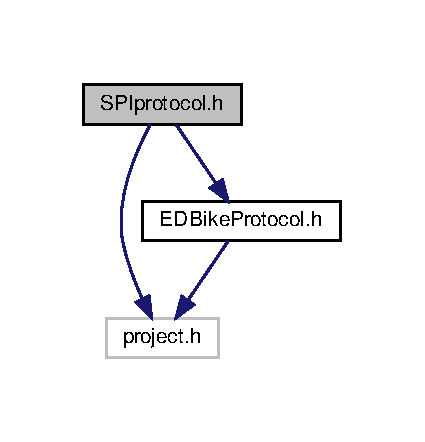
\includegraphics[width=204pt]{SPIprotocol_8h__incl}
\end{center}
\end{figure}
This graph shows which files directly or indirectly include this file\+:
\nopagebreak
\begin{figure}[H]
\begin{center}
\leavevmode
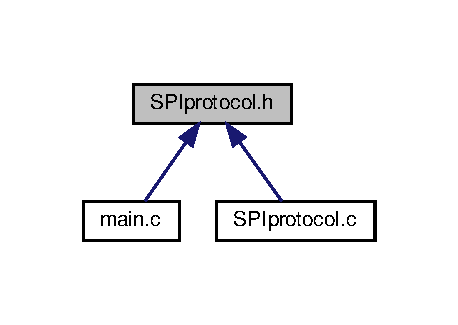
\includegraphics[width=220pt]{SPIprotocol_8h__dep__incl}
\end{center}
\end{figure}
\subsection*{Functions}
\begin{DoxyCompactItemize}
\item 
void \hyperlink{SPIprotocol_8h_a43827de2fc968bbd1b3081e66c606cf8}{extract\+From\+Buffer} (uint8\+\_\+t $\ast$speed, uint8\+\_\+t $\ast$distance, uint8\+\_\+t $\ast$buffer)
\begin{DoxyCompactList}\small\item\em Funktion til at uddrage information fra en buffer Henter speed og distance fra rx bufferen. \end{DoxyCompactList}\item 
uint8\+\_\+t \hyperlink{SPIprotocol_8h_affe5db7b5f6fb00785f2e52d8b5462f0}{error\+Check\+With\+Odd\+Parity} (uint8\+\_\+t $\ast$buffer, uint8\+\_\+t length\+Of\+Buffer)
\begin{DoxyCompactList}\small\item\em Funktion til check af paritets bit. Checker tx/rx buffere for paritets bit. \end{DoxyCompactList}\item 
void \hyperlink{SPIprotocol_8h_a9f7556559e84f123b72eefce42c02710}{create\+Parity\+Bits} (uint8\+\_\+t $\ast$buffer, uint8\+\_\+t length\+Of\+Buffer)
\begin{DoxyCompactList}\small\item\em Funktion til kreering af paritets bits Laver paritet bits til en tx/rx buffer. \end{DoxyCompactList}\end{DoxyCompactItemize}


\subsection{Detailed Description}
Funktions prototyper til håndtering af S\+P\+I-\/protokol. 

Indeholder funktions prototyperne til \hyperlink{SPIprotocol_8c}{S\+P\+Iprotocol.\+c}

\begin{DoxyAuthor}{Author}
Kristian Lau Jespersen 
\end{DoxyAuthor}
\begin{DoxyRefDesc}{Bug}
\item[\hyperlink{bug__bug000009}{Bug}]Ingen kendte bugs. \end{DoxyRefDesc}


\subsection{Function Documentation}
\mbox{\Hypertarget{SPIprotocol_8h_a9f7556559e84f123b72eefce42c02710}\label{SPIprotocol_8h_a9f7556559e84f123b72eefce42c02710}} 
\index{S\+P\+Iprotocol.\+h@{S\+P\+Iprotocol.\+h}!create\+Parity\+Bits@{create\+Parity\+Bits}}
\index{create\+Parity\+Bits@{create\+Parity\+Bits}!S\+P\+Iprotocol.\+h@{S\+P\+Iprotocol.\+h}}
\subsubsection{\texorpdfstring{create\+Parity\+Bits()}{createParityBits()}}
{\footnotesize\ttfamily void create\+Parity\+Bits (\begin{DoxyParamCaption}\item[{uint8\+\_\+t $\ast$}]{buffer,  }\item[{uint8\+\_\+t}]{length\+Of\+Buffer }\end{DoxyParamCaption})}



Funktion til kreering af paritets bits Laver paritet bits til en tx/rx buffer. 


\begin{DoxyParams}{Parameters}
{\em buffer} & \\
\hline
{\em length\+Of\+Buffer} & \\
\hline
\end{DoxyParams}
\mbox{\Hypertarget{SPIprotocol_8h_affe5db7b5f6fb00785f2e52d8b5462f0}\label{SPIprotocol_8h_affe5db7b5f6fb00785f2e52d8b5462f0}} 
\index{S\+P\+Iprotocol.\+h@{S\+P\+Iprotocol.\+h}!error\+Check\+With\+Odd\+Parity@{error\+Check\+With\+Odd\+Parity}}
\index{error\+Check\+With\+Odd\+Parity@{error\+Check\+With\+Odd\+Parity}!S\+P\+Iprotocol.\+h@{S\+P\+Iprotocol.\+h}}
\subsubsection{\texorpdfstring{error\+Check\+With\+Odd\+Parity()}{errorCheckWithOddParity()}}
{\footnotesize\ttfamily uint8\+\_\+t error\+Check\+With\+Odd\+Parity (\begin{DoxyParamCaption}\item[{uint8\+\_\+t $\ast$}]{buffer,  }\item[{uint8\+\_\+t}]{length\+Of\+Buffer }\end{DoxyParamCaption})}



Funktion til check af paritets bit. Checker tx/rx buffere for paritets bit. 


\begin{DoxyParams}{Parameters}
{\em buffer} & \\
\hline
{\em length\+Of\+Buffer} & \\
\hline
\end{DoxyParams}
\begin{DoxyReturn}{Returns}
1 eller 0 alt efter om der er en parity error. 
\end{DoxyReturn}
\mbox{\Hypertarget{SPIprotocol_8h_a43827de2fc968bbd1b3081e66c606cf8}\label{SPIprotocol_8h_a43827de2fc968bbd1b3081e66c606cf8}} 
\index{S\+P\+Iprotocol.\+h@{S\+P\+Iprotocol.\+h}!extract\+From\+Buffer@{extract\+From\+Buffer}}
\index{extract\+From\+Buffer@{extract\+From\+Buffer}!S\+P\+Iprotocol.\+h@{S\+P\+Iprotocol.\+h}}
\subsubsection{\texorpdfstring{extract\+From\+Buffer()}{extractFromBuffer()}}
{\footnotesize\ttfamily void extract\+From\+Buffer (\begin{DoxyParamCaption}\item[{uint8\+\_\+t $\ast$}]{speed,  }\item[{uint8\+\_\+t $\ast$}]{distance,  }\item[{uint8\+\_\+t $\ast$}]{buffer }\end{DoxyParamCaption})}



Funktion til at uddrage information fra en buffer Henter speed og distance fra rx bufferen. 


\begin{DoxyParams}{Parameters}
{\em speed} & \\
\hline
{\em distance} & \\
\hline
{\em buffer} & \\
\hline
\end{DoxyParams}

\hypertarget{UART_8c}{}\section{U\+A\+R\+T.\+c File Reference}
\label{UART_8c}\index{U\+A\+R\+T.\+c@{U\+A\+R\+T.\+c}}


funktions implementeringer til U\+A\+RT  


{\ttfamily \#include \char`\"{}U\+A\+R\+T.\+h\char`\"{}}\newline
Include dependency graph for U\+A\+R\+T.\+c\+:
\nopagebreak
\begin{figure}[H]
\begin{center}
\leavevmode
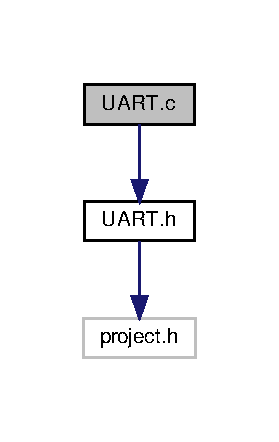
\includegraphics[width=134pt]{UART_8c__incl}
\end{center}
\end{figure}
\subsection*{Functions}
\begin{DoxyCompactItemize}
\item 
\mbox{\Hypertarget{UART_8c_a2cb50cd9b95f3b32212def6b17da3931}\label{UART_8c_a2cb50cd9b95f3b32212def6b17da3931}} 
void \hyperlink{UART_8c_a2cb50cd9b95f3b32212def6b17da3931}{init\+U\+A\+RT} ()
\begin{DoxyCompactList}\small\item\em Init funktion til U\+A\+RT Initierer U\+A\+RT ved at ved hjælp af U\+A\+R\+T\+\_\+\+Start() A\+PI funktionen, og initierering interrupt handlers. \end{DoxyCompactList}\end{DoxyCompactItemize}


\subsection{Detailed Description}
funktions implementeringer til U\+A\+RT 

Indeholder implementeringer af funktionerne fra \hyperlink{UART_8h_source}{U\+A\+R\+T.\+h}

\begin{DoxyAuthor}{Author}
Kristian Lau Jespersen 

Jonathan Hartvigsen Juncker 
\end{DoxyAuthor}
\begin{DoxyRefDesc}{Bug}
\item[\hyperlink{bug__bug000010}{Bug}]Ingen kendte bugs. \end{DoxyRefDesc}

\hypertarget{wheelSensor_8h}{}\section{wheel\+Sensor.\+h File Reference}
\label{wheelSensor_8h}\index{wheel\+Sensor.\+h@{wheel\+Sensor.\+h}}


Indeholder Funktions implementeringer til wheel revolution sensor.  


{\ttfamily \#include $<$project.\+h$>$}\newline
{\ttfamily \#include $<$math.\+h$>$}\newline
{\ttfamily \#include $<$stdio.\+h$>$}\newline
{\ttfamily \#include $<$stdlib.\+h$>$}\newline
Include dependency graph for wheel\+Sensor.\+h\+:
\nopagebreak
\begin{figure}[H]
\begin{center}
\leavevmode
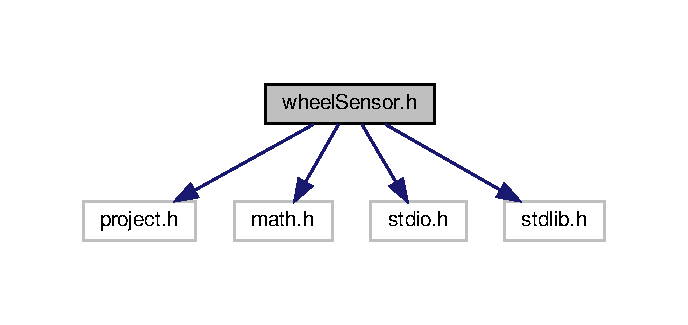
\includegraphics[width=330pt]{wheelSensor_8h__incl}
\end{center}
\end{figure}
This graph shows which files directly or indirectly include this file\+:
\nopagebreak
\begin{figure}[H]
\begin{center}
\leavevmode
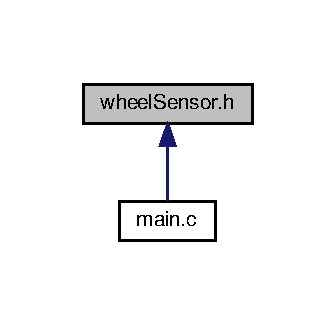
\includegraphics[width=161pt]{wheelSensor_8h__dep__incl}
\end{center}
\end{figure}
\subsection*{Functions}
\begin{DoxyCompactItemize}
\item 
\mbox{\Hypertarget{wheelSensor_8h_a0d17b051af54d6f930860c7df88d8419}\label{wheelSensor_8h_a0d17b051af54d6f930860c7df88d8419}} 
void \hyperlink{wheelSensor_8h_a0d17b051af54d6f930860c7df88d8419}{init\+Wheel\+Sensor} ()
\begin{DoxyCompactList}\small\item\em Init funktion til Wheel\+Sensor Initierer wheel\+Sensor ved at ved hjælp af wheel\+Tick\+Timer\+\_\+\+Start() A\+PI funktionen, og initierering interrupt handlers. \end{DoxyCompactList}\item 
double \hyperlink{wheelSensor_8h_a77ce324fe6e22324d32f62c0fd529b02}{Wheel\+Radius\+To\+Metres} (uint8)
\begin{DoxyCompactList}\small\item\em Funktion til ændring af radius i cm til radius i m Når funktionen modtager en radius i cm ændre den det til m, så radiussen kan bruges til udregning af hjulets omkreds. \end{DoxyCompactList}\item 
double \hyperlink{wheelSensor_8h_a5124c7c730314a9c8f45460158fa0c32}{calc\+Wheel\+Circ} (double)
\begin{DoxyCompactList}\small\item\em Funktion til udregning af hjulets omkreds Når funktionen modtager en radius i m. udregner den hjulets omkreds i km, så det kan bruges til udregning af hastighed og distance kørt. \end{DoxyCompactList}\item 
double \hyperlink{wheelSensor_8h_acf2e76c364916dd1e63f11f79a9a97d8}{calc\+Distance} (int, double)
\begin{DoxyCompactList}\small\item\em Funktion til udregning af distance kørt. Funktionen \hyperlink{wheelSensor_8h_acf2e76c364916dd1e63f11f79a9a97d8}{calc\+Distance()}, indeholder funktionaliteten til distanceberegninger. Til dette anvendes parameteren wheel\+Circumference. \hyperlink{wheelSensor_8h_acf2e76c364916dd1e63f11f79a9a97d8}{calc\+Distance()} multiplicerer antal omdrejninger detekteret med omkredsen af hjulet, opbevaret i variablen wheel\+Circumference. \hyperlink{wheelSensor_8h_acf2e76c364916dd1e63f11f79a9a97d8}{calc\+Distance()} returnerer distanceværdien i enheden km. \end{DoxyCompactList}\item 
double \hyperlink{wheelSensor_8h_aea8e5e1a1ead23be679149302ec1d72e}{calc\+Speed} (double counter\+\_\+value, double circumference)
\begin{DoxyCompactList}\small\item\em Funktion til udregning af hastighed. Til beregning af hastigheden tages der udgangspunkt i hjulets omkreds samt tiden siden sidste gang, der blev foretaget en omdrejning af hjulet. \end{DoxyCompactList}\item 
void \hyperlink{wheelSensor_8h_a69517cf5b2648ce4a6dd5dbe49ed8420}{set\+Speed\+To\+Zero} (uint8 $\ast$)
\begin{DoxyCompactList}\small\item\em Funktion til at sætte hastigheden til 0. Sætter hastigheden til 0, efter 3 sekunder ved hjælp af en timer. \end{DoxyCompactList}\item 
void \hyperlink{wheelSensor_8h_ac9a707cad628e31ba45190ca497e60ab}{reset\+Speed\+Timer} ()
\begin{DoxyCompactList}\small\item\em Funktion til reset af Wheel\+Tick\+Timer Skriver til timerens counter, for at reset den. \end{DoxyCompactList}\end{DoxyCompactItemize}


\subsection{Detailed Description}
Indeholder Funktions implementeringer til wheel revolution sensor. 

Funktions og interrupt prototyper til Wheel revolution sensor.

Indeholder implementeringer af funktionerne fra \hyperlink{wheelSensor_8h}{wheel\+Sensor.\+h}

\begin{DoxyAuthor}{Author}
Jonathan Hartvigsen Juncker 
\end{DoxyAuthor}
\begin{DoxyRefDesc}{Bug}
\item[\hyperlink{bug__bug000012}{Bug}]Ingen kendte bugs. \end{DoxyRefDesc}


Indeholder prototyperne til interrupt handlers som relaterer til S\+PI og funktions prototyperne til wheel\+Sensor.\+c

\begin{DoxyAuthor}{Author}
Jonathan Hartvigsen Juncker 
\end{DoxyAuthor}
\begin{DoxyRefDesc}{Bug}
\item[\hyperlink{bug__bug000013}{Bug}]Ingen kendte bugs. \end{DoxyRefDesc}


\subsection{Function Documentation}
\mbox{\Hypertarget{wheelSensor_8h_acf2e76c364916dd1e63f11f79a9a97d8}\label{wheelSensor_8h_acf2e76c364916dd1e63f11f79a9a97d8}} 
\index{wheel\+Sensor.\+h@{wheel\+Sensor.\+h}!calc\+Distance@{calc\+Distance}}
\index{calc\+Distance@{calc\+Distance}!wheel\+Sensor.\+h@{wheel\+Sensor.\+h}}
\subsubsection{\texorpdfstring{calc\+Distance()}{calcDistance()}}
{\footnotesize\ttfamily double calc\+Distance (\begin{DoxyParamCaption}\item[{int}]{,  }\item[{double}]{ }\end{DoxyParamCaption})}



Funktion til udregning af distance kørt. Funktionen \hyperlink{wheelSensor_8h_acf2e76c364916dd1e63f11f79a9a97d8}{calc\+Distance()}, indeholder funktionaliteten til distanceberegninger. Til dette anvendes parameteren wheel\+Circumference. \hyperlink{wheelSensor_8h_acf2e76c364916dd1e63f11f79a9a97d8}{calc\+Distance()} multiplicerer antal omdrejninger detekteret med omkredsen af hjulet, opbevaret i variablen wheel\+Circumference. \hyperlink{wheelSensor_8h_acf2e76c364916dd1e63f11f79a9a97d8}{calc\+Distance()} returnerer distanceværdien i enheden km. 


\begin{DoxyParams}{Parameters}
{\em Wheelticks} & Antallet af omdrejninger som hjulet har lavet.\\
\hline
{\em wheel\+Circumference} & Hjulets omkreds i km.\\
\hline
\end{DoxyParams}
\begin{DoxyReturn}{Returns}
Distance Antal km cyklen har kørt 
\end{DoxyReturn}
\mbox{\Hypertarget{wheelSensor_8h_aea8e5e1a1ead23be679149302ec1d72e}\label{wheelSensor_8h_aea8e5e1a1ead23be679149302ec1d72e}} 
\index{wheel\+Sensor.\+h@{wheel\+Sensor.\+h}!calc\+Speed@{calc\+Speed}}
\index{calc\+Speed@{calc\+Speed}!wheel\+Sensor.\+h@{wheel\+Sensor.\+h}}
\subsubsection{\texorpdfstring{calc\+Speed()}{calcSpeed()}}
{\footnotesize\ttfamily double calc\+Speed (\begin{DoxyParamCaption}\item[{double}]{counter\+\_\+value,  }\item[{double}]{circumference }\end{DoxyParamCaption})}



Funktion til udregning af hastighed. Til beregning af hastigheden tages der udgangspunkt i hjulets omkreds samt tiden siden sidste gang, der blev foretaget en omdrejning af hjulet. 


\begin{DoxyParams}{Parameters}
{\em Time} & Tiden siden sidste hjul omdrejning\\
\hline
{\em wheel\+Circumference} & hjulets omkreds i km.\\
\hline
\end{DoxyParams}
\begin{DoxyReturn}{Returns}
Speed returnerer en Hhastighed i km/t 
\end{DoxyReturn}
\mbox{\Hypertarget{wheelSensor_8h_a5124c7c730314a9c8f45460158fa0c32}\label{wheelSensor_8h_a5124c7c730314a9c8f45460158fa0c32}} 
\index{wheel\+Sensor.\+h@{wheel\+Sensor.\+h}!calc\+Wheel\+Circ@{calc\+Wheel\+Circ}}
\index{calc\+Wheel\+Circ@{calc\+Wheel\+Circ}!wheel\+Sensor.\+h@{wheel\+Sensor.\+h}}
\subsubsection{\texorpdfstring{calc\+Wheel\+Circ()}{calcWheelCirc()}}
{\footnotesize\ttfamily double calc\+Wheel\+Circ (\begin{DoxyParamCaption}\item[{double}]{ }\end{DoxyParamCaption})}



Funktion til udregning af hjulets omkreds Når funktionen modtager en radius i m. udregner den hjulets omkreds i km, så det kan bruges til udregning af hastighed og distance kørt. 


\begin{DoxyParams}{Parameters}
{\em radius} & radius i m.\\
\hline
\end{DoxyParams}
\begin{DoxyReturn}{Returns}
hjulets omkreds returnerer hjulets omkreds i km. 
\end{DoxyReturn}
\mbox{\Hypertarget{wheelSensor_8h_ac9a707cad628e31ba45190ca497e60ab}\label{wheelSensor_8h_ac9a707cad628e31ba45190ca497e60ab}} 
\index{wheel\+Sensor.\+h@{wheel\+Sensor.\+h}!reset\+Speed\+Timer@{reset\+Speed\+Timer}}
\index{reset\+Speed\+Timer@{reset\+Speed\+Timer}!wheel\+Sensor.\+h@{wheel\+Sensor.\+h}}
\subsubsection{\texorpdfstring{reset\+Speed\+Timer()}{resetSpeedTimer()}}
{\footnotesize\ttfamily void reset\+Speed\+Timer (\begin{DoxyParamCaption}{ }\end{DoxyParamCaption})}



Funktion til reset af Wheel\+Tick\+Timer Skriver til timerens counter, for at reset den. 

\mbox{\Hypertarget{wheelSensor_8h_a69517cf5b2648ce4a6dd5dbe49ed8420}\label{wheelSensor_8h_a69517cf5b2648ce4a6dd5dbe49ed8420}} 
\index{wheel\+Sensor.\+h@{wheel\+Sensor.\+h}!set\+Speed\+To\+Zero@{set\+Speed\+To\+Zero}}
\index{set\+Speed\+To\+Zero@{set\+Speed\+To\+Zero}!wheel\+Sensor.\+h@{wheel\+Sensor.\+h}}
\subsubsection{\texorpdfstring{set\+Speed\+To\+Zero()}{setSpeedToZero()}}
{\footnotesize\ttfamily void set\+Speed\+To\+Zero (\begin{DoxyParamCaption}\item[{uint8 $\ast$}]{ }\end{DoxyParamCaption})}



Funktion til at sætte hastigheden til 0. Sætter hastigheden til 0, efter 3 sekunder ved hjælp af en timer. 


\begin{DoxyParams}{Parameters}
{\em uint8$\ast$} & speed\\
\hline
\end{DoxyParams}
\begin{DoxyReturn}{Returns}
Speed returnerer en hastighed på 0 km/t 
\end{DoxyReturn}
\mbox{\Hypertarget{wheelSensor_8h_a77ce324fe6e22324d32f62c0fd529b02}\label{wheelSensor_8h_a77ce324fe6e22324d32f62c0fd529b02}} 
\index{wheel\+Sensor.\+h@{wheel\+Sensor.\+h}!Wheel\+Radius\+To\+Metres@{Wheel\+Radius\+To\+Metres}}
\index{Wheel\+Radius\+To\+Metres@{Wheel\+Radius\+To\+Metres}!wheel\+Sensor.\+h@{wheel\+Sensor.\+h}}
\subsubsection{\texorpdfstring{Wheel\+Radius\+To\+Metres()}{WheelRadiusToMetres()}}
{\footnotesize\ttfamily double Wheel\+Radius\+To\+Metres (\begin{DoxyParamCaption}\item[{uint8}]{ }\end{DoxyParamCaption})}



Funktion til ændring af radius i cm til radius i m Når funktionen modtager en radius i cm ændre den det til m, så radiussen kan bruges til udregning af hjulets omkreds. 


\begin{DoxyParams}{Parameters}
{\em radius} & radius i cm.\\
\hline
\end{DoxyParams}
\begin{DoxyReturn}{Returns}
radius radius i m. 
\end{DoxyReturn}

%--- End generated contents ---

% Index
\backmatter
\newpage
\phantomsection
\clearemptydoublepage
\addcontentsline{toc}{chapter}{Index}
\printindex

\end{document}
